\scanpage{45}
D'après le théor. d'Artin--Schreier--Witt, on a
\[
H^1(A,\mathbb Z/p)\simeq H^1(A,\underline O_A)^{\unsure{(\varphi)|(p)}}_{\deleted{\unsure{\varphi}}}
\]
éléments de $H^1(A,\underline O_A)$ tels que
\[Fx=x\]
\[
H^1(A,\mathbb Z/p^n)\simeq H^1(A,\underline O_A(W_n))^{\unsure{(\varphi)|(p)}}
\]
--- $H^1(A,\underline O_A(W_n))$ tels que
\[Fx=x\]
\[
\vcenter{\hbox{\begingroup
\setbox0=\hbox{$\displaystyle \operatorname{Hom}(\pi_1^p(A),\mathbb Z_p)\simeq H^1(A,\deleted{\unsure{\mathbb Q_p}}\mathbb Z_p)\simeq H^1(A,\mathbb W)^{\unsure{(\varphi)|(p)}}_{\deleted{\unsure{\varphi}}}$}
\dimen0=\wd0 \advance\dimen0 by 18pt
\dimen2=\ht0 \advance\dimen2 by \dp0 \advance\dimen2 by 16pt
\rlap{\raisebox{\dimexpr-\dp0-8pt\relax}{%
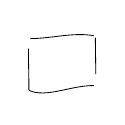
\begin{tikzpicture}[x={\dimexpr\dimen0/1020\relax},y={\dimexpr-\dimen2/145\relax},line width=.3pt]
\path[use as bounding box] (0,0) rectangle (1020,145);
\draw (40,23) .. controls (350,23) and (680,9) .. (982,17);
\draw (12,44) .. controls (11,77) and (20,110) .. (18,132);
\draw (21,132) .. controls (270,149) and (650,121) .. (981,122);
\draw (1002,21) -- (1009,98);
\end{tikzpicture}}}%
\kern9pt\box0\kern9pt\endgroup}}
\]
\deleted{\unsure{on}} \inserted{d'où} \deleted{\inserted{\unsure{a}}} on déduit un \deleted{accouplement} isomorphisme
\[
\vcenter{\hbox{\begingroup
\setbox0=\hbox{$\displaystyle \deleted{\pi_1^p(A)\times H^1(A,\mathbb W)_s\longrightarrow\mathbb Z_p}$}
\dimen0=\wd0 \advance\dimen0 by 18pt
\dimen2=\ht0 \advance\dimen2 by \dp0 \advance\dimen2 by 16pt
\rlap{\raisebox{\dimexpr-\dp0-8pt\relax}{%
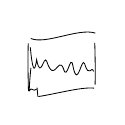
\begin{tikzpicture}[x={\dimexpr\dimen0/770\relax},y={\dimexpr-\dimen2/140\relax},line width=.3pt]
\path[use as bounding box] (0,0) rectangle (770,140);
\draw (35,22) .. controls (200,35) and (570,0) .. (756,11);
\draw (6,32) .. controls (2,63) and (4,103) .. (9,129);
\draw (120,140) .. controls (310,135) and (600,120) .. (744,123);
\draw (750,31) .. controls (756,65) and (756,95) .. (754,116);
\draw (30,40) .. controls (48,79) and (75,99) .. (100,65) .. controls (145,108) and (180,54) .. (212,68) .. controls (300,116) and (340,56) .. (400,83) .. controls (440,112) and (478,50) .. (505,77) .. controls (559,128) and (600,58) .. (636,73) .. controls (690,105) and (710,75) .. (737,89);
\draw (36,82) .. controls (25,101) and (15,126) .. (19,128) .. controls (45,119) and (60,132) .. (100,125);
\draw (105,122) -- (114,140);
\end{tikzpicture}}}%
\kern9pt\box0\kern9pt\endgroup}}
\]
\[
\vcenter{\hbox{\begingroup
\setbox0=\hbox{$\displaystyle \deleted{\operatorname{Hom}_{\mathrm{cont}}(\pi_1^p(A),\Lambda)\simeq H^1(A,\mathbb W)_s}$}
\dimen0=\wd0 \advance\dimen0 by 18pt
\dimen2=\ht0 \advance\dimen2 by \dp0 \advance\dimen2 by 16pt
\rlap{\raisebox{\dimexpr-\dp0-8pt\relax}{%
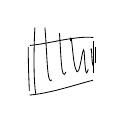
\begin{tikzpicture}[x={\dimexpr\dimen0/900\relax},y={\dimexpr-\dimen2/190\relax},line width=.3pt]
\path[use as bounding box] (0,0) rectangle (900,190);
\draw (29,49) .. controls (260,45) and (620,22) .. (858,27);
\draw (8,53) .. controls (7,103) and (16,145) .. (22,174);
\draw (24,186) .. controls (300,181) and (630,157) .. (853,145);
\draw (858,37) -- (858,126);
\draw (880,53) -- (880,97);
\draw (94,0) .. controls (79,61) and (76,148) .. (106,183);
\draw (225,0) .. controls (258,76) and (250,163) .. (318,144);
\draw (415,15) .. controls (437,74) and (437,153) .. (500,122);
\draw (558,37) .. controls (575,0) and (585,95) .. (630,115) .. controls (680,149) and (720,37) .. (738,66) .. controls (750,105) and (756,143) .. (791,115);
\draw (824,62) .. controls (842,46) and (832,99) .. (856,105);
\end{tikzpicture}}}%
\kern9pt\box0\kern9pt\endgroup}}
\]
qui est une dualité \deleted{\unsure{de}} de $\mathbb Z_p$-modules libres de type fini

D'autre part, utilisant encore le fait que tout revêtement de $A$ est une variété abélienne, on trouve aussi
\[\boxed{\pi_1^p(A)\simeq T_p(A)}\]
d'où en les composant
\[
\vcenter{\hbox{\begingroup
\setbox0=\hbox{$\displaystyle T_p(A)\times H^1(A,\mathbb W)^{\unsure{(\varphi)|(p)}}\longrightarrow\mathbb Z_p$}
\dimen0=\wd0 \advance\dimen0 by 18pt
\dimen2=\ht0 \advance\dimen2 by \dp0 \advance\dimen2 by 16pt
\rlap{\raisebox{\dimexpr-\dp0-8pt\relax}{%
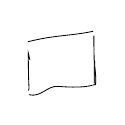
\begin{tikzpicture}[x={\dimexpr\dimen0/795\relax},y={\dimexpr-\dimen2/190\relax},line width=.3pt]
\path[use as bounding box] (0,0) rectangle (795,190);
\draw (0,39) .. controls (310,20) and (500,23) .. (755,10);
\draw (25,89) -- (7,70) .. controls (8,106) and (8,135) .. (16,168) -- (8,173);
\draw (13,185) .. controls (160,193) and (220,160) .. (350,162) .. controls (510,165) and (650,165) .. (748,159);
\draw (764,22) .. controls (763,60) and (771,85) .. (768,153);
\draw (773,91) .. controls (775,122) and (778,145) .. (779,157) -- (754,158);
\draw (774,107) .. controls (789,134) and (787,147) .. (784,157) -- (778,158);
\end{tikzpicture}}}%
\kern9pt\box0\kern9pt\endgroup}}
\]
qui est une dualité de $\mathbb Z_p$-modules libres de type fini.

\deleted{qu'on peut aussi écrire} \unsure{donc|d'où} on déduit
\[
\vcenter{\hbox{\begingroup
\setbox0=\hbox{$\displaystyle \operatorname{Hom}_{\mathrm{cont}}(T_p(A),\deleted{\unsure{\mathbb Z_\ell|\Lambda}}W_\infty(k))\simeq H^1(A,\mathbb W)_s$}
\dimen0=\wd0 \advance\dimen0 by 18pt
\dimen2=\ht0 \advance\dimen2 by \dp0 \advance\dimen2 by 16pt
\rlap{\raisebox{\dimexpr-\dp0-8pt\relax}{%
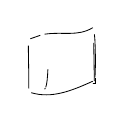
\begin{tikzpicture}[x={\dimexpr\dimen0/910\relax},y={\dimexpr-\dimen2/180\relax},line width=.3pt]
\path[use as bounding box] (0,0) rectangle (910,180);
\draw (35,29) -- (166,20);
\draw (224,17) .. controls (470,10) and (660,24) .. (861,0);
\draw (9,47) .. controls (10,91) and (18,133) .. (14,159);
\draw (47,170) .. controls (320,186) and (580,165) .. (860,140);
\draw (873,40) -- (881,140);
\draw (879,20) .. controls (887,7) and (904,88) .. (889,130);
\draw (861,146) -- (895,146) -- (896,132);
\draw (224,161) -- (233,158);
\draw (239,156) .. controls (254,148) and (263,130) .. (267,109);
\end{tikzpicture}}}%
\kern9pt\box0\kern9pt\endgroup}}
\]
\margin{44}
